\chapter[Neutrino telescopes]{Breaking the cross section degeneracy: neutrino telescopes}
\label{ch:NT}

The presence of dark matter (DM) in the Solar neighbourhood provides the opportunity to directly detect its scattering in terrestrial detectors. This may give us a handle on both the DM mass and speed distribution, providing we use a range of detector materials, as we have investigated in Chapter \ref{ch:Poly}. However, the finite energy thresholds of direct detection experiments means that we cannot probe the entire range of DM speeds. With no sensitivity to low speed WIMPs, we also cannot know what fraction of WIMPs are probed by the experiments, resulting in a loss of sensitivity to the DM interaction cross section.

The local DM population may also scatter with nuclei in the Sun, becoming gravitationally captured if enough energy is lost in the interaction \cite{Press:1985,Silk:1985, Gaisser:1986, Srednicki:1987, Griest:1987}. These can then annihilate in the Sun and produce neutrinos, which may be observed at neutrino telescope (NT) experiments such as IceCube. Importantly, capture occurs preferentially for WIMPs with low energy or, equivalently, low speed. Such a signal at a NT experiment would provide complementary sensitivity to the low speed WIMP population, hopefully breaking the degeneracy in the DM interaction cross section. 

In this chapter, we discuss the formalism for calculating the solar capture rate, as well as the processes of neutrino production, propagation and detection. We then test the binned speed parametrisation (discussed in Chapter \ref{ch:Speed}) and the polynomial parametrisation (presented in Chapter \ref{ch:Poly}) using both direct detection and IceCube mock data. In particular, we test the ability of these data sets - in conjunction with parametrisations of the speed distributions - to constrain the DM interaction cross sections in addition to the DM mass. We note that due to the high abundance of spin-1/2 hydrogen in the Sun, we must consider both spin-independent (SI) and spin-dependent (SD) couplings.

In Sec.~\ref{sec:NT:formalism}, we describe the IceCube event rate formalism. We then propose several particle physics and astrophysical benchmarks for the dark matter population in Sec.~\ref{sec:NT:benchmarks}. Section~\ref{sec:NT:experiments} describes the experimental parameters used in the analysis, with particular attention to the isotopic composition of detectors and the SD form factors. In the remaining sections, we consider reconstructions of particle physics parameters first without IceCube data (Sec.~\ref{sec:NT:withoutIC}) and then with IceCube data (Sec.~\ref{sec:NT:withIC}), before discussing the prospects for reconstructing $f(v)$ itself (Sec.~\ref{sec:NT:speeddist}).

\section{Neutrino telescope formalism}

Calculation of the expected spectrum of neutrinos at an NT experiment can be broadly decomposed into 3 contributions. The first is the rate at which WIMPs scatter and are captured in the Sun. The second is the subsequent thermalisation of the solar WIMP population and their eventual annihilation into neutrinos. Third, we must model the detection of neutrinos at the IceCube detector. We now consider each of these in turn, focusing on the first, as this is where the WIMP cross sections and speed distribution enter into the calculation.

\subsection{Solar capture}

In calculating the solar capture rate, we follow closely the treatment of Gould \cite{Gould:1987,Gould:1992}. WIMPs are captured by the Sun when they elastically scatter off one of its constituent nuclei and end up with a speed lower than the solar escape velocity (which at the surface is equal to \(v_{\textrm{esc}}^\odot = 617.5 \kms\) \cite{Kaufmann:1991}). These WIMPs then enter bound orbits intersecting the Sun, ensuring further scatters with solar nuclei during subsequent passes. WIMPs may become unbound in subsequent scatters (this possibility will be discussed later) but typically lose energy until they collect and thermalise around the Sun's core.

\begin{figure}[h!]
    \centering
    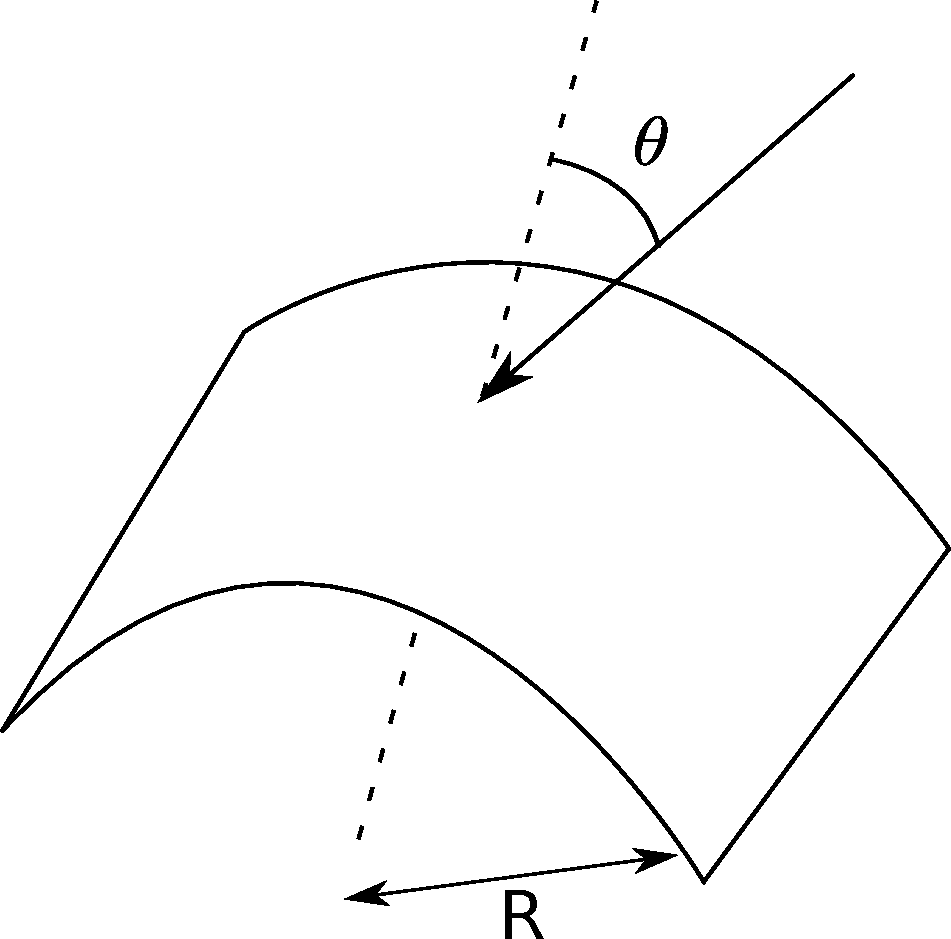
\includegraphics[width=0.4\textwidth]{NT/Surface.pdf}
\caption[Geometry of WIMPs impinging on the Sun]{Illustration of the geometry of WIMPs impinging on the Sun}
\label{fig:NT:geometry}
\end{figure}

In order to calculate this `first-scatter' probability, we consider a thin spherical shell of radius $R$, large enough that the gravitational field at $R$ is negligible. This geometry is illustrated schematically in Fig.~\ref{fig:NT:geometry}. The number density of WIMPs with speed $v$ is $n_\chi f_1(v) \,\mathrm{d}v$. Because of the spherical symmetry of the problem, we can assume that the WIMP velocity distribution is isotropic without loss of generality. The fraction of WIMPs with direction $\cos \theta \rightarrow \cos \theta + \textrm{d} \cos \theta$ relative to the perpendicular direction is $\frac{1}{2} \textrm{d}\cos\theta$ (normalised over all values of $\cos \theta$). The WIMP speed perpendicular to the surface is given by $v \cos\theta$, meaning that the WIMP flux inward through the surface (per unit area) can be written:
\begin{equation}
\frac{1}{2} f_1(v) v \cos\theta \,\textrm{d}v \,\textrm{d}\cos\theta = \frac{1}{4} f_1(v) v \,\textrm{d}v \,\textrm{d}\cos^2\theta \,, \qquad \theta \in [0, \frac{\pi}{2}]\,.
\end{equation}
We change variables to angular momentum per unit mass, $ J = R v \sin\theta $, and integrate over all area elements on the surface of the shell to obtain the inward WIMP flux per unit time
\begin{equation}
4 \pi R^2 \frac{1}{4}f_1(v) v \, \textrm{d}v \frac{\textrm{d}J^2}{R^2 v^2}.
\end{equation}

\note{[***Missing a factor of the WIMP density***]}
We now consider an inner shell of radius $r$ and thickness $dr$. If the escape velocity at the shell is $\vesc(r)$, then a WIMP with speed $v$ at infinity will have speed $w = \sqrt{v^2 + \vesc^2(r)}$ at this inner shell. The total time the WIMP spends in the shell is

\begin{equation}
\frac{\textrm{d}l}{w} = \frac{2}{w \cos \theta} \Theta(1 - \sin\theta) \, \textrm{d}r = \frac{2}{w}\left[ 1 - \left(\frac{J}{rw}\right)^2\right]^{-1/2} \Theta(rw - J) \, \textrm{d}r\,,
\end{equation}
where the Heaviside step function $\Theta$ appears because the WIMP crosses the shell either twice or not at all. If the rate per unit time at which a single WIMP travelling at velocity \(w\) is scattered down to a speed less than the escape speed \(\vesc\) is given by \(\Omega^{-}_{\vesc,i}(w)\), then we can write the WIMP capture rate per unit time per unit velocity as
\begin{align}
&2\pi \, \textrm{d}r \frac{f_1(v)}{v}\,\textrm{d}v \frac{\ScatRate}{w}  \, \int_{0}^{(rw)^2} \left[ 1 - \left(\frac{J}{rw}\right)^2\right]^{-1/2} \, \textrm{d}(J^2) \nonumber\\&\qquad= 4 \pi r^2 \, \textrm{d}r \frac{f_1(v)}{v}\, \textrm{d}v w \ScatRate\,.
\end{align}

The `first scatter' rate is then given by integrating over the radius of the Sun:
\begin{equation}
C_{\odot} = \frac{\rho_0}{m_\chi} \int_{0}^{R_{\odot}} \textrm{d}r \sum_i \dbd{C_i}{V} 4 \pi r^{2},
\end{equation}
where the capture rate per unit shell volume is
\begin{equation}
\label{eq:NT:dCdV}
\dbd{C_i}{V} = \int_{0}^{v_{\textrm{max}}} \textrm{d}v \frac{f_1(v)}{v} w \ScatRate\,.
\end{equation}
The index \(i\) labels the various nuclei in the Sun. The integration limit is
\begin{equation}
v_{\textrm{max}} = \frac{\sqrt{4m_\chi m_{N_i}}}{m_\chi - m_{N_i}}\vesc\,.
\end{equation}
WIMPs above this speed cannot lose enough energy in a recoil to drop below the escape speed.

We now calculate the factor $\ScatRate$, which gives the rate per unit time at which a single WIMP travelling at velocity \(w\) is scattered down to a speed less than the escape speed \(\vesc\). This rate can be written as:
\begin{equation}
\ScatRate = \Phi_\chi N_T \sigma_{\vesc}\,
\end{equation}
where \(\Phi_\chi N_T\) is the WIMP flux multiplied by the number of target nuclei. For a single WIMP and a number density of nuclei \(n_N\), this becomes \( \Phi_\chi N_T = w n_N\). The cross-section for the process \(\sigma_{\vesc}\) is given by:
\begin{equation}
\label{eq:NT:sigma}
\sigma_{\vesc}  = \int_{E_{\vesc}}^{E_\textrm{max}} \dbd{\sigma}{E_R} \, \textrm{d}E_R\,
\end{equation}
where \(E_R = \Delta E\) is the energy lost by the scattering WIMP. The limits of integration run from the minimum energy loss required to reduce the WIMP speed below \vesc,
\begin{equation}
E_{\vesc} = \frac{m_\chi}{2}(w^2 - \vesc^2) = \frac{m_\chi}{2}v^2\,,
\end{equation}
to the maximum possible energy loss in the collision,
\begin{equation}
E_\textrm{max} = \frac{2 \mu_{\chi N}^2}{m_N} w^2\,.
\end{equation}

As in the direct detection case, we can decompose the differential cross section into SI and SD components. While all of the constituent elements of the Sun are sensitive to the SI interaction, only spin-1/2 Hydrogen is sensitive to SD scattering. The differential cross section is therefore given by

\begin{equation}
\dbd{\sigma}{E_R} = \frac{m_{N_i}}{2\mu_{\chi p}^2 v^2}
\begin{cases}
\sigmapsi + \sigmapsd & \textrm{ for } A = 1 \\
\sigmapsi A_i^2 F_i^2(E_R) & \textrm{ for } A > 1 \,.
\end{cases}
\end{equation}
No form factor is needed for Hydrogen ($A=1$), which consists of only a single nucleon. For the remaining nuclei, approximate the form factor as \cite{Gould:1987}
\begin{equation}
F^2_i(E_R) = \exp(-E_R/E_i); \qquad E_i = \frac{3}{2m_{N_i} R_i^2}\,,
\end{equation}
where $R_i$ is the nuclear radius (see Sec.~\ref{}). These expressions allow Eq.~\ref{eq:NT:sigma} to be calculated analytically and introduce an error in the total capture rate of only a few percent.

\note{Might need some plots illustrating capture rates...}

In addition to the effects which have already been described, we can also consider a number of other factors which may impact the WIMP capture rate. The fact that nuclei in the Sun have a finite temperature has been neglected so far. However, detailed calculation \cite{Press:1985,Gould:1987} shows that this gives a correction to the capture rate of only around 1\% for WIMP masses above around 10 GeV. The gravitational influence of other bodies in the Solar system may also have an impact. For example, Peter \cite{Peter:2009} found that WIMPs whose bound orbits reach out as far as Jupiter can be perturbed by the planet and become unbound. This leads to so-called \textit{Jupiter depletion} for WIMPs heavier than around 1 TeV. However, a recent study by Sivertsson and Edsj\"{o} \cite{Sivertsson:2012} showed using Liouville's theorem that such depletion processes must be accompanied by an inverse diffusion process. The net result is that for Solar capture we can treat the WIMP population as being free.

\note{Gould:1991}

\subsection{Evolution of the WIMP population}

Once a WIMP has scattered to below the escape speed at a given solar position, it will be in a bound orbit and will enter the population of WIMPs captured by the Sun. Subsequent scatters with the nuclei in the Sun will lead to an approximately thermal distribution. There are then two processes which will tend to deplete this population: WIMP evaporation and annihilation. \note{Look up \cite{Krauss:1986}.} 

Evaporation occurs when WIMPs scatter into the high speed tail of the thermal distribution, above the Solar escape velocity, and become unbound. It has been shown that for a WIMP mass of around 4 GeV, the evaporation timescale is approximately equal to the lifetime of the Sun ($\sim4.7$ billion years) \cite{Gould:1987b}. For WIMPs significantly heavier than this, the evaporation rate is negligible compared to the capture rate. For WIMPs lighter than this, the tail of the Maxwell-Boltzmann distribution lying above the escape velocity becomes significant and evaporation can no longer be neglected \cite{Busoni:2013b}. As we will see, the IceCube detector is sensitive to WIMPs with masses above around $m_\chi > 20 \textrm{ GeV} $, meaning that we can safely ignore the effects of evaporation.

The population of WIMPs will also undergo annihilation (either with their anti-particle partners or with themselves if they are Majorana particles). The evolution of the total number $N(t)$ of WIMPs in the Sun can then be written as \cite{Griest:1987}:

\begin{equation}
\dbd{N}{t} = C_c - \frac{1}{2}C_a N^2 - C_e N\,.
\end{equation}
The parameter $C_c$ is the total capture rate and the parameters $C_a$ and $C_e$ determine the annihilation and evaporation rates. As we have discussed, we can safely negelect evaporation, so we set $C_e$ to zero. The parameter $C_a$ and therefore the annihilation rate will depend on the velocity-averaged annihilation cross section $\langle \sigma v \rangle$ which is \textit{a priori} unknown. Over a long period of time, equilibrium between the capture and annihilation will be achieved and a steady state scenario for the WIMP population will be reached. This timescale is set by the equilibration time $\tau = 1/\sqrt{C_c C_a}$. If this is sufficiently short compared to the lifetime of the Sun, the WIMP population will currently be in equilibrium with the annihilation rate $\Gamma_a$ set by the capture rate as

\begin{equation}
\Gamma_a = \frac{1}{2}C_a\,.
\end{equation}

Crucially, in this case, the annihilation rate no longer depends on the unknown annihilation cross section, but is related only to the WIMP-nucleus scattering cross sections. We will assume in the rest of this chapter that the annihilation cross section is sufficiently high that the equilibrium assumption is valid.

Standard Model (SM) particles are produced in these annihilations, the majority of which cannot escape the Sun. However, some of these particles may decay to neutrinos or neutrinos may be produced directly in the WIMP annihilation. These neutrinos can escape the Sun and may be detected at neutrino telescope experiments on Earth. It is important to account for the production and propagation of neutrinos in the dense medium of the Sun, as well as the propagation of these neutrinos from the Sun to the Earth \cite{Blennow:2008}. The spectrum of neutrinos reaching Earth can be written as \note{Wait but this doesn't take into account the propagation does it...?}

\begin{equation}
\dbd{N_\nu}{E_\nu} = \frac{\Gamma_a}{4\pi D^2}\sum_f B_f \dbd{N_\nu^f}{E_\nu}\,,
\end{equation}
where $D$ is the Earth-Sun distance, $\mathrm{d}N_\nu^f/\mathrm{d}E_\nu$ is the neutrino spectrum produced in the Sun for a particular final state $f$ and $B_f$ is the branching ratio into that final state. The branching ratios will depend on the specific form of the dark matter interactions with baryons. Typically, in order to set constraints on the WIMP interaction cross sections, we consider annihilation into only one channel at a time, assuming $B_f = 1$ for that particular channel during the analysis. Finally, the neutrino spectrum produced in the annihilation $\mathrm{d}N_\nu^f/\mathrm{d}E_\nu$ can be obtained using particle physics event generators (such as \textsc{Pythia} \cite{Sjostrand:1994}) and propagated to Earth using neutrino Monte Carlo simulations (such as WimpSim \cite{Blennow:2008}).


\note{Sub-section on propagation??? What should go in which section???}

\subsection{Detection}

Neutrinos which escape the Sun can be detected at terrestrial NT experiments \cite{Adrian-Martinez:2013,Aartsen:2013b}. We focus in this work on the IceCube experiment \cite{Aartsen:2013b}, which can detect the \v{C}erenkov radiation produced by high energy particles traveling through ice. Muon neutrinos interact via charged-current interactions in the ice to produce relativistic muons. These in turn produce \v{C}erenkov light, which is collected by digital optical modules (DOMs). The amount and pattern of lit DOMs allows the energy and direction of the incoming neutrino to be reconstructed \note{with varying degrees of accuracy}. 

\todo{Talk about showers vs cascades}

\todo{Talk about the energy threshold}

\todo{Talk about DeepCore! \cite{Abbasi:2012}} 

\todo{Talk about the event-level likelihoods paper... - base it on that!}

\section{Complementarity with direct detection}

The complementarity between direct detection and NT data has been studied in the past \cite{Arina:2013}. In particular, the high abundance of hydrogen can help to constrain the spin-dependent cross section and, even in cases where no signal is observed at IceCube, limits from NT experiments can help to reduce the size of the allowed parameter space. Here, we explore further this complementarity by looking at the range of speeds which are probed by NT experiments.

As can be from Eq.~\ref{eq:NT:dCdV}, WIMPs with speeds from $v=0$ up to $v=v_\textrm{max}$ have the possibility of being captured by the Sun. In particular, with increasing WIMP speed the capture probability decreases, \note{Not even sure if this is true}, further suppressed by loss of coherence in the SI case. As pointed out in Ref.~\cite{Choi:2013}, direct detection experiments probe a complementary range of the WIMP speed distribution, defined by the energy range of the WIMP search window. If the ranges of speeds probed by direct detection and NT experiments overlaps, this means that the entire WIMP speed distribution can be probed.

In Fig.~\ref{fig:NT:speedoverlap}, we show the WIMP speeds to which two experiments are sensitive as a function of WIMP mass. As a blue band, we show the region probed by a Xenon direction detection experiment. The lower and upper limits of the band are set by $v_\textrm{min}(\Emin)$ and $v_\textrm{min}(\Emax)$, where \Emin and \Emax define the extent of the WIMP signal window. In this chapter, we consider a window of $[5,45]$ keV \cite{}. WIMPs with speeds above the blue band still contribute to the overall event rate (so there is still some sensitivity to them). However, there is no information on the \textit{shape} of the distribution at higher speeds, as we are not sensitive to the event spectrum above \Emax.


\begin{figure}[t]
  \centering
  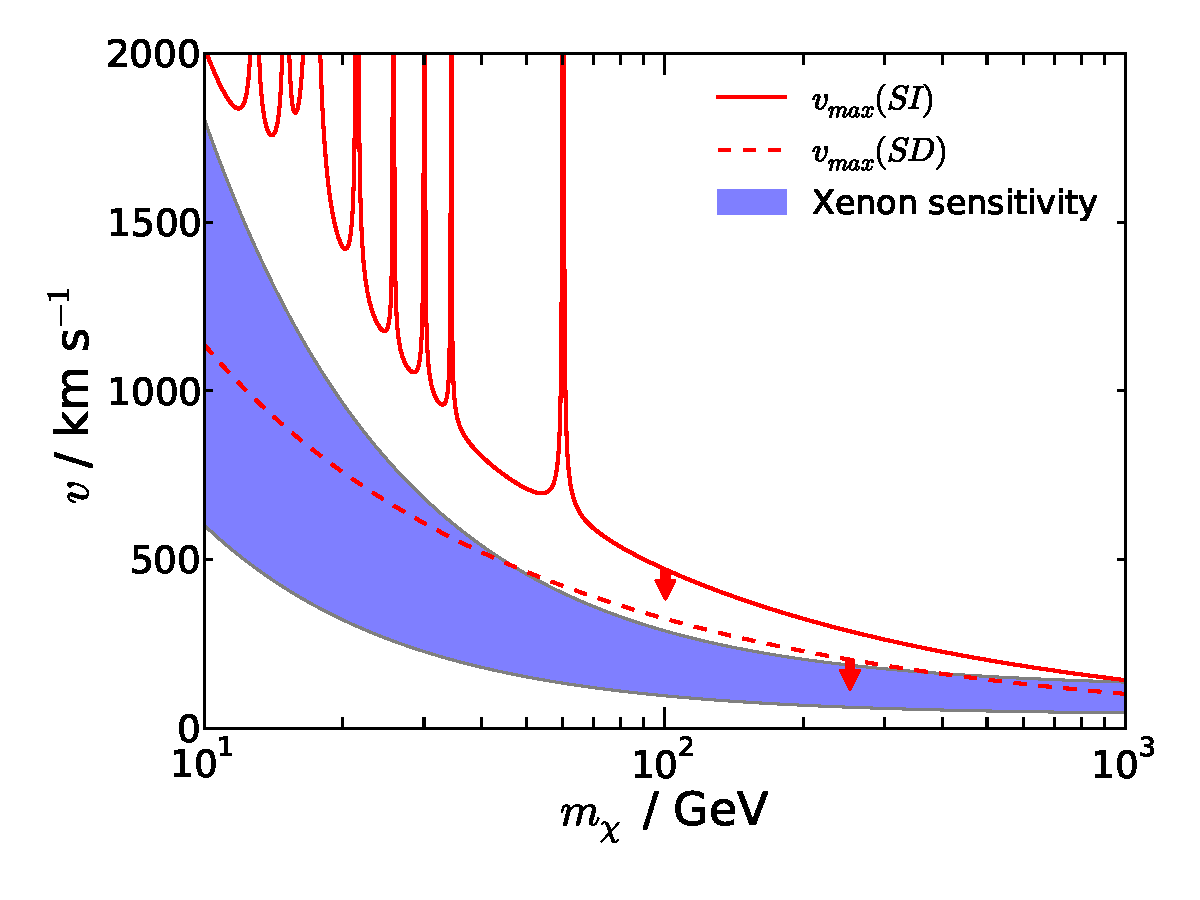
\includegraphics[trim=0.8cm 0.9cm 0cm 0cm, clip,width=0.75\textwidth]{NT/SpeedOverlap.pdf}
  \caption[Speed sensitivity ranges of solar capture and direct detection experiments as a function of WIMP mass]{Sensitivity ranges of solar capture and direct detection experiments. We show as a blue band the range of speeds to which a Xenon detector is sensitive using an energy window of $[5,45]$ keV. The maximum speed to which solar WIMP capture is sensitive is shown as a solid (dashed) red line for SI (SD) interactions (see the text for more details).}
  \label{fig:NT:speedoverlap}
\end{figure}

Also shown in Fig.~\ref{fig:NT:speedoverlap} are the values of $v_\textrm{max}$ involved in the Solar capture rate for SI and SD interactions. In the SD case, the maximum speed is set by the hydrogen mass $m_H$:

\begin{equation}
v_{\textrm{max}} = \frac{\sqrt{4m_\chi m_H}}{m_\chi - m_H}\vesc\,.
\end{equation}
The escape speed \vesc depends on radius within the Sun so we use an average value, weighted by the hydrogen density as a function of radius. In the SI case, the situation is more complex, as more than one nucleus contributes to the capture rate. We therefore consider the average value of $v_\textrm{max}$ weighted by the mass fraction $f_i$ of each species

\begin{equation}
\langle v_{\textrm{max}} \rangle = \sum_i f_i \frac{\sqrt{4m_\chi m_{N_i}}}{m_\chi - m_{N_i}}\vesc\,,
\end{equation}
where again \vesc is evaluated at the average radius of each species $i$.

In the SD case, the decreasing value of $v_\textrm{max}$ with $\mchi$ reflects the kinematics of the $\chi-H$ interaction. As the WIMP mass increases, scattering with hydrogen becomes less effecient at transferring energy. In the SI case, the value of $v_\textrm{max}$ is typically higher because the WIMP is closer in mass to the heavier nuclei in the Sun. However, there is still a significant SI interaction with hydrogen and the same decay with $\mchi$ is observed as in the SD case. In addition, there are resonances in $v_\textrm{max}$, corresponding to perfect mass matching between the WIMP and one of the nuclei in the Sun. In these cases, energy transfer is highly efficient and WIMPs of any speed can scatter into bound orbits.

The key point of Fig.~\ref{fig:NT:speedoverlap} is that in both the SI and SD dominated cases, $v_\textrm{max}$ never falls below the lower limit of the blue band. This means that the combination of NT and direct detection data should provide sensitivity to the full range of WIMP speeds over a range of masses. The level of sensitivity may vary with WIMP speed, due for example to a falling capture contribution from higher speeds or form factor suppression in direct detection experiments. However, in principle, we can probe the full WIMP speed distribution and hopefully break the degeneracy in the cross section described in Chapter~\ref{ch:Poly}. The inclusion of data sets from additional direct detection experiments should only improve this sensitivity.

\note{Need a linking paragraph here...}



\section{Current limits?}

\section{Benchmarks and experiments}
\label{sec:NT:experiments}
In order to test these parametrisations and determine how well the WIMP parameters can be recovered, we generate mock data sets for a set of hypothetical direct detection experiments as well as for IceCube. We show in Table~\ref{tab:NT:Experiments} the parameters used in this work for three direct detection experiments chosen to mimic next-generation detectors currently in development. Each experiment is described by the range of nuclear recoil energies it is sensitive to and the total exposure (the product of the fiducial detector mass, the exposure time and the experimental and operating efficiencies). We also include a gaussian energy resolution of $\sigma_E = 1 \textrm{ keV}$ and a flat background rate of $10^{-7}$ events/kg/day/keV.

\note{NB: `While the exact reconstructions, and in particular the uncertainties, will depend on the values used for the experiments and benchmarks, the general method is gooood.'}

We divide the energy range of each experiment into bins and generate Asimov data \cite{Cowan:2013} by setting the observed number of events in each bin equal to the expected number of events. While this cannot correspond to a physical realisation of data as the observed number of events will be non-integer, it allows us to disentangle the effects of Poisson fluctuations from the properties of the parametrisations under study.

\begin{table}[t]
  \setlength{\extrarowheight}{3pt}
  \begin{center}
%\begin{sideways}
	\begin{tabular}{cm{2.75cm}m{2.5cm}m{2.75cm}}
        \hline\hline
	Experiment & Energy Range (keV) & Exposure (ton-yr) & Energy bin width (keV) \\
        \hline
	Xenon &  5-45 & 1.0 & 2.0 \\
	Argon &  30-100 & 1.0 & 2.0 \\
	Germanium  & 10-100 & 0.3 & 2.0 \\
        \hline\hline
	\end{tabular}
%\end{sideways}
  \end{center}
\label{tab:NT:Experiments}
\caption[Summary of parameters for mock direct detection experiments used in Chapter~\ref{ch:NT}]{Summary of parameters for mock direct detection experiments. All experiments have a constant energy resolution of $\sigma_E = 1 \textrm{ keV}$ and a flat background rate of $10^{-7}$ events/kg/day/keV. \note{Probably need some references/justification for some of these values.}}
\end{table}

To generate neutrino telescope data, we consider the IceCube 86-string configuration. We use an exposure time of 900 days (corresponding to five 180 day austral winter observing seasons, as in Ref.~\cite{Arina:2013}). We use an angular cut around the solar position $\phi_\textrm{cut} = 3\,^{\circ}$. This results in approximately 217 background events over the full exposure. As with the direct detection experiments, we set the observed number of events equal to the expected number of signal plus background events. We use only the observed number of events as data and not the energies of the individual events. While event-level likelihood methods have previously been developed \cite{Scott:2012} for use with IceCube 22-string data \cite{Abbasi:2009}. However, a similar analysis has not been performed for IceCube-86. In particular, the probability distributions for the number of lit digital optical modules (DOMs) as a function of neutrino energy are not yet available for IceCube-86. Nonetheless, using the number of observed events at IceCube is a first step towards using neutrino telescope data to help constrain the WIMP speed distribution.

\subsection{Benchmarks}
\label{sec:NT:benchmarks}
We use four benchmark models to generate mock data sets, which are summarised in Table~\ref{tab:benchmarks}. In all cases, we use an SI WIMP proton cross section of $\sigmapsi = 10^{-45} \textrm{ cm}^2$ and SD cross-section of $\sigmapsd = 2 \times 10^{-40} \textrm{ cm}^2$, both of which are close to the current best exclusion limits \cite{Akerib:2014, Aprile:2013}. For simplicity, we assume that the WIMP-proton and WIMP-neutron couplings are equal in both the SI and SD cases. We could allow the ratio of these couplings to vary as free parameters, but this would introduce additional degeneracies into the analysis. Here we focus on the degeneracy associated with the WIMP speed distribution.

Benchmark A represents an intermediate mass WIMP which annihilates to $W^{+}W^{-}$, which is similar to benchmark B used by Ref.~\cite{Arina:2013}. As we will see, even with this intermediate mass there is already a strong degeneracy in the reconstructed WIMP mass. We therefore choose not to consider a benchmark model with higher mass, which would result in an even poorer sensitivity to the reconstructed WIMP mass. We do, however, consider a lighter WIMP in benchmark C, which annihilates to $\nu_\mu \bar{\nu}_\mu$. The IceCube detector (with DeepCore) is sensitive to WIMPs with masses down to about 20 GeV \cite{}. We therefore use a 30 GeV WIMP mass, as WIMPs much lighter than this cannot feasibly be detected by IceCube.

\begin{table*}[t]
  \setlength{\extrarowheight}{3pt}
  \begin{center}
%\begin{sideways}
	\begin{tabular}{ccccccc}
        \hline\hline
	Benchmark & $m_\chi \textrm{ (GeV)}$ & $\sigma^p_{SI} \textrm{ (cm}^2\textrm{)}$ & $\sigma^p_{SD} \textrm{ (cm}^2\textrm{)}$ & Speed distribution & Decay channel \\
	\hline
        A & 100 & $10^{-45}$ & $2 \times 10^{-40}$ & SHM & $W^{+}W^{-}$ \\
        B & 100 & $10^{-45}$ & $2 \times 10^{-40}$ & SHM+DD & $W^{+}W^{-}$ \\
        C & 30  & $10^{-45}$ & $2 \times 10^{-40}$ & SHM & $\nu_\mu \bar{\nu}_\mu$ \\
        D & 30  & $10^{-45}$ & $2 \times 10^{-40}$ & SHM+DD & $\nu_\mu \bar{\nu}_\mu$ \\
        \hline\hline
	\end{tabular}
%\end{sideways}
  \end{center}
\label{tab:NT:benchmarks}
\caption[Summary of benchmarks used in Chapter~\ref{ch:NT}]{Summary of benchmarks. In all cases, we consider only isospin conserving interactions (i.e. $f_p = f_n$ and $a_p = a_n$).}
\end{table*}

Benchmarks A and C assume an SHM speed distribution described by $v_\textrm{lag} = 230 \kms$ and $\sigma_v = 163 \kms$. Benchmarks B and D assume the same particle physics parameters as A and C respectively, but assuming an SHM distribution with a moderate dark disk overdensity (SHM+DD). We model the dark disk as contributing an additional 30\% dark matter density to the SHM, with parameters $v_\textrm{lag} = 50 \kms$ and $\sigma_v = 50 \kms$ \cite{}. As shown in Ref.~\cite{Choi:2013}, the capture rate in the Sun is not strongly dependent on variations in the shape of $f(v)$ (such as the differences between distribution functions extracted from different N-body simulations). However, significant enhancement of the capture rate can be achieved with the presence of a low speed dark disk, which we investigate using these two astrophysical benchmarks.

%%%%%Hmmm...the speed distribution probed by the earth is not precisely the same as the one probed by the Sun because of the Earth's motion round the Sun...but that's not a big factor

\subsection{Parameter sampling}
\label{sec:NT:sampling}
We perform parameter scans using a modified version of the publicly available \textsc{MultiNest 3.6} package \cite{Feroz:2007, Feroz:2008, Feroz:2014}. This allows us to map out the likelihood $\mathcal{L}(\theta)$ for the model parameters $\theta$.  We use $N_\textrm{live} = 20000$ live points in the scans and a tolerance of $10^{-4}$. We show in Table~\ref{tab:NT:priors} the priors on the various model parameters used in this work.

\begin{table}
  \setlength{\extrarowheight}{3pt}
  \begin{center}
%\begin{sideways}
	\begin{tabular}{ccc}
        \hline\hline
	Parameter & Prior range & Prior type \\
        \hline
        $m_\chi$ (GeV) & 10-1000 & log-flat \\
        $\sigma^p_{SI} \textrm{ (cm}^2\textrm{)}$ & $10^{-48} - 10^{-42}$ & log-flat \\
        $\sigma^p_{SD} \textrm{ (cm}^2\textrm{)}$ & $10^{-43} - 10^{-37}$ & log-flat \\
        Polynomial coefficients $\left\{a_k\right\}$ & $-20 - 20$ & linear-flat \\
        Bin heights $\left\{\hat{g}_k\right\}$ & $0-1$ & simplex \\
        \hline\hline
        \end{tabular}
%\end{sideways}
  \end{center}
\label{tab:NT:priors}
\caption[Summary of \textsc{MultiNest} priors used in Chapter~\ref{ch:NT}]{Summary of \textsc{MultiNest} priors used in this work. The `simplex' priors are described in Sec.~\ref{sec:sampling}.}
\end{table}

\note{Need to actually mention/include something about the parametrisations in this chapter...}
Due to the normalisation condition on the bin heights (given in Eq.~\ref{eq:normalisation}), we must sample these parameters from `simplex' priors. That is, we must uniformly sample $\left\{\hat{g}_2,...,\hat{g}_N\right\}$ such that they sum to less than one and then fix $\hat{g}_1$ as
\begin{equation}
\hat{g_1} = 1 - \sum_{i = 2}^N \hat{g}_i \,.
\end{equation}
This is achieved by sampling the bin heights from a dirichlet distribution \note{probably give more details on this}. The ellipsoidal sampling performed by \textsc{MultiNest} becomes increasingly inefficient as the number of bins $N$ increases, as the volume of the parameter space for which Eq.~\ref{eq:normalisation} is satisfied becomes very small. Instead, we sample the $\hat{g}_i$ from the dirichlet distribution, subject to the hard constraints $\hat{g}_i \leq c_i$. The limits $c_i$ are set by the maximum value of $\hat{g}_i$ in the current set of live points, providing an approximation to the isolikelihood contour from which to sample. This allows us to sample from the remaining prior volume much more efficiently. \note{Clarify...} The remaining (non-bin) parameters are sampled using ellipsoidal sampling as usual.

We use a total of 10 bins in the binned parameterisation (9 free parameters, with one fixed by normalisation), which should allow us to obtain a close approximation to the rapidly varying SHM+DD distribution. In the polynomial $\ln f(v)$ parametrisation, we use 5 basis polynomials (4 free coefficients, with one fixed by normalisation). This is because the parameter space is significantly larger than for the binned case and would require a much larger number of live points to accurately map the likelihood using 10 parameters. As we will see, using 5 basis functions still allows a wide range of speed distributions to be explored and can provide a good fit to the data. With increasing numbers of events, it would be feasible to increase the number of basis functions and more precisely parametrisate the form of the speed distribution.

The likelihood function we use for each experiment is:

\begin{equation}
\mathcal{L}(\theta) = \left(\prod_{i = 1, N_\textrm{bins}} \frac{(N_e^i)^{N_o^i}}{(N_o^i)!}e^{-N_e^i}\right)^{1/N_\textrm{bins}}\,,
\end{equation}
where the signal region is divided into $N_\textrm{bins}$ bins with $N_e^i$ events expected and $N_o^i$ events observed in the $i$th bin. We weight the likelihood by a factor $1/N_\textrm{bins}$ so that the direct detection experiments (for which there are a large number of bins in energy) receive the same weight as the IceCube experiment (for which $N_\textrm{bins} = 1$). \note{Give explicit forms for the likelihood?} The total likelihood is then the product over all experiments under consideration.

\section{Reconstructions without IceCube}
\label{sec:NT:withoutIC}

We show first reconstructions without using data from IceCube. These results are distinct from the results of Chapter~\ref{ch:Poly} in that we are also including a contribution to the rate from spin-dependent interactions. As we shall see, this has a strong impact on the reconstructions.

\begin{figure}[!ht]
  \centering
  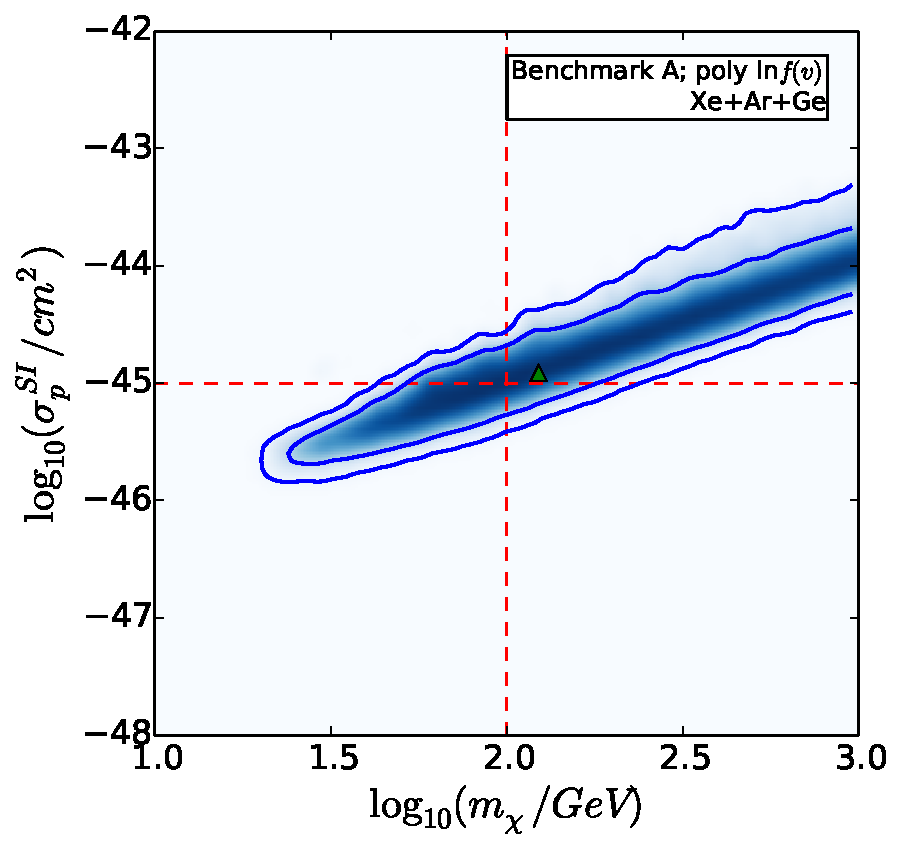
\includegraphics[width=0.32\textwidth]{NT/BenchmarkA_poly_noIC-mx_sigsi.pdf}
  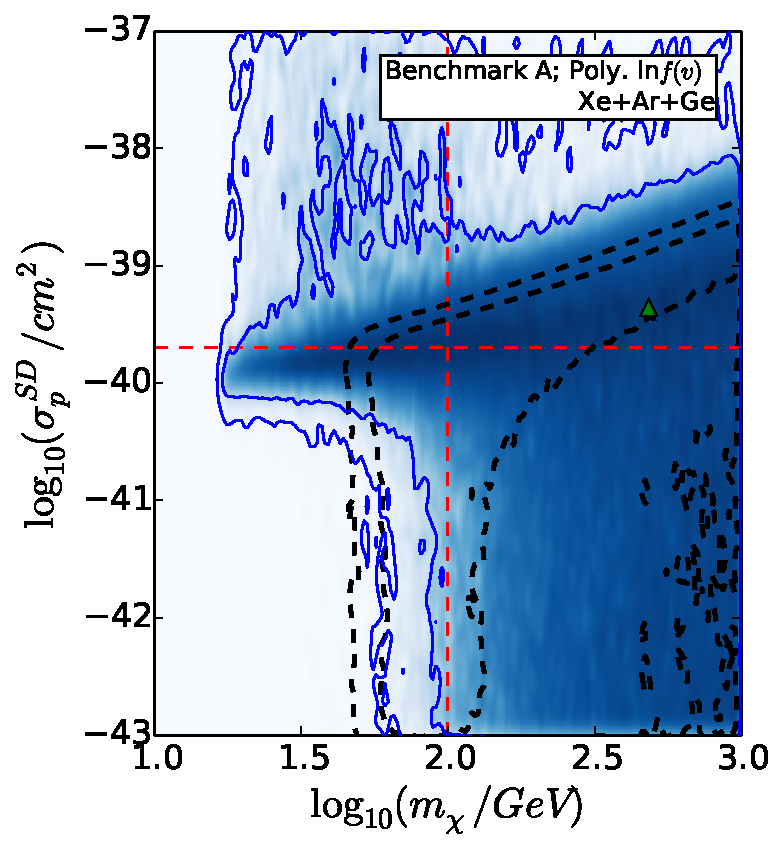
\includegraphics[width=0.32\textwidth]{NT/BenchmarkA_poly_noIC-mx_sigsd.pdf}
  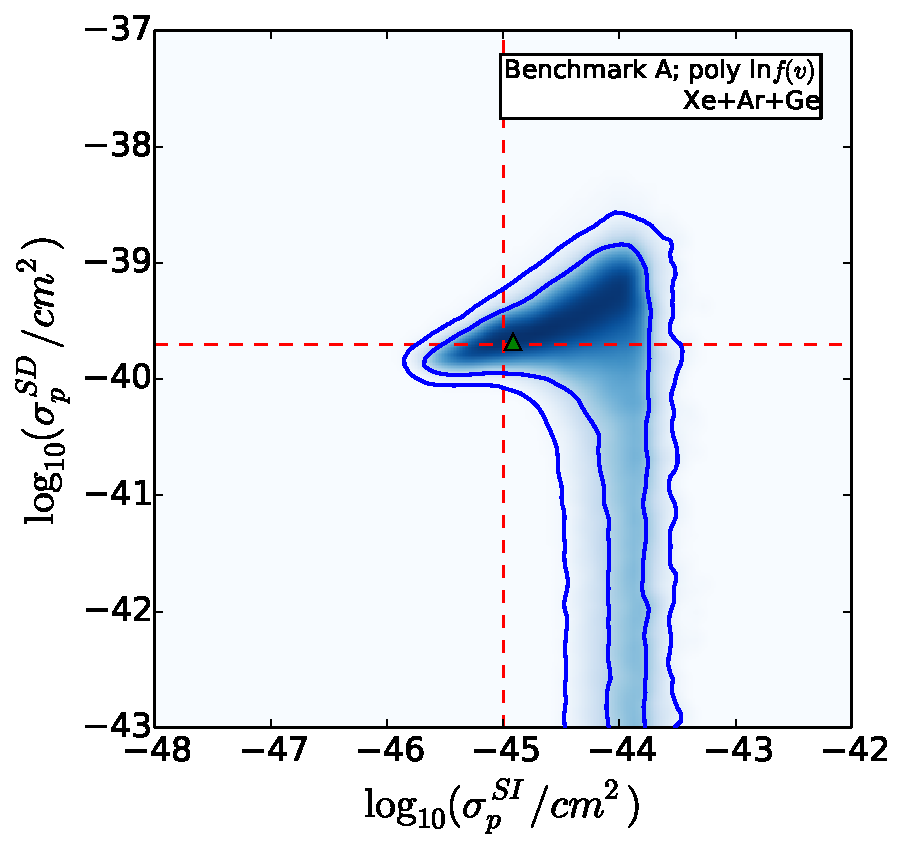
\includegraphics[width=0.32\textwidth]{NT/BenchmarkA_poly_noIC-sigsi_sigsd.pdf}

  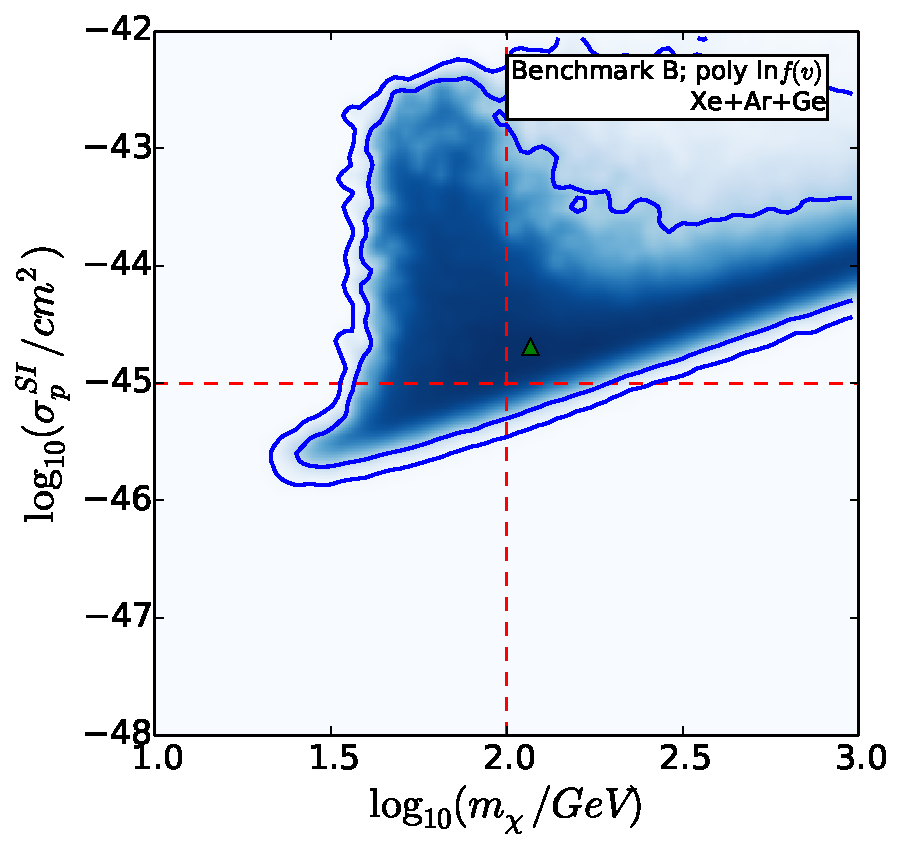
\includegraphics[width=0.32\textwidth]{NT/BenchmarkB_poly_noIC-mx_sigsi.pdf}
  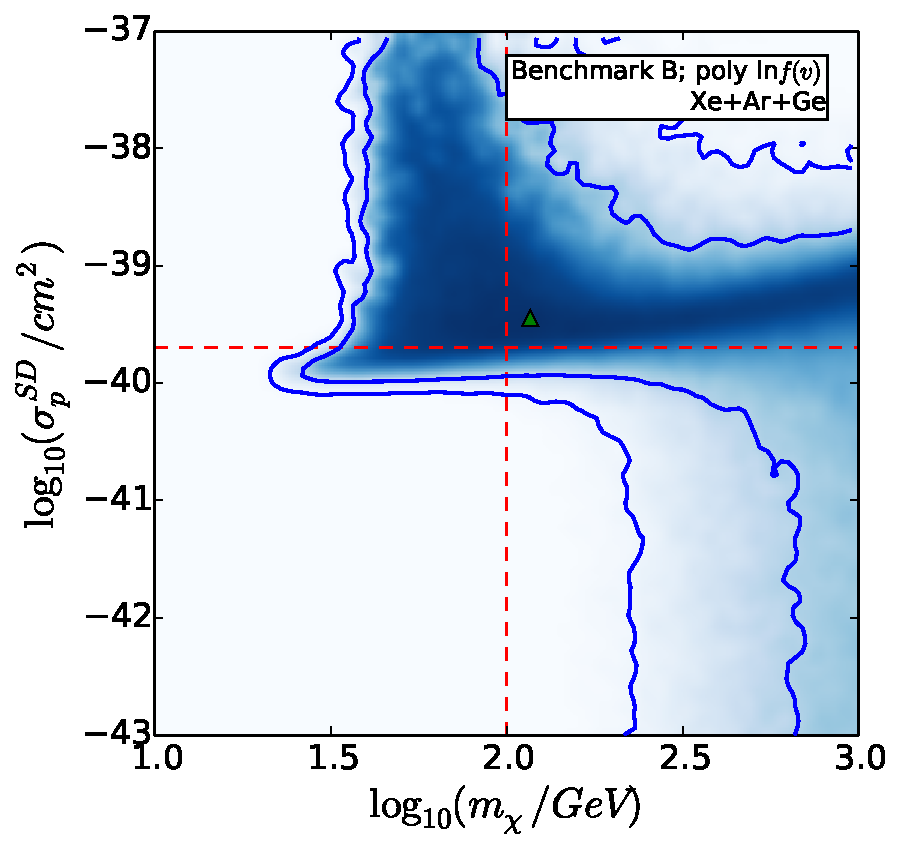
\includegraphics[width=0.32\textwidth]{NT/BenchmarkB_poly_noIC-mx_sigsd.pdf}
  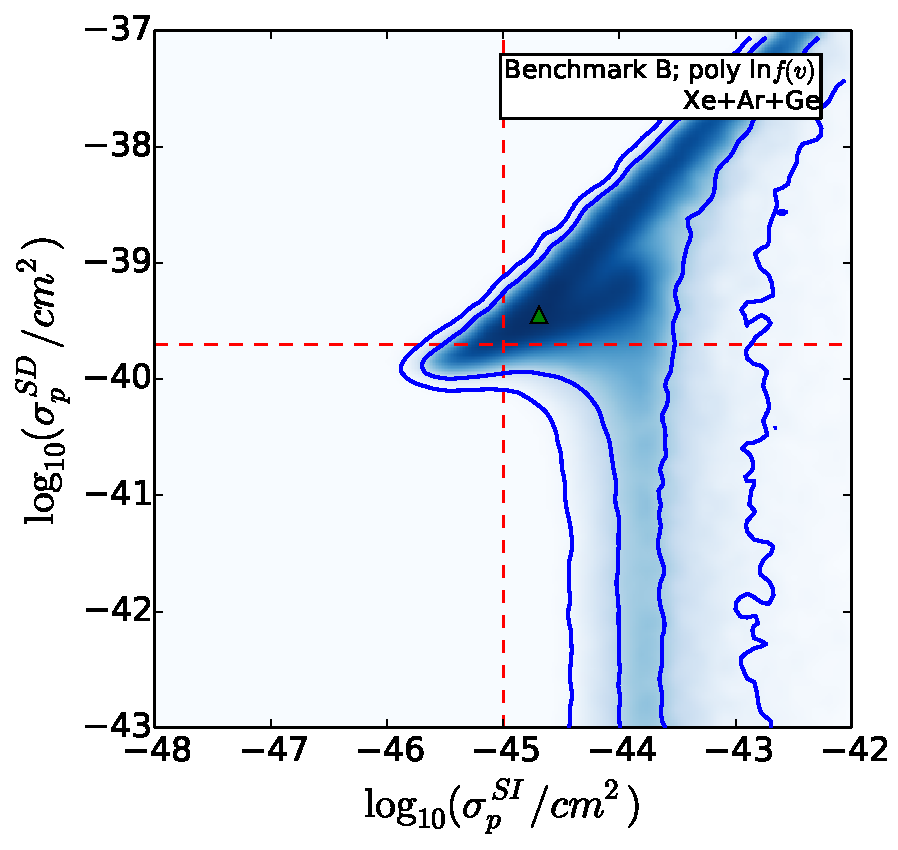
\includegraphics[width=0.32\textwidth]{NT/BenchmarkB_poly_noIC-sigsi_sigsd.pdf}

  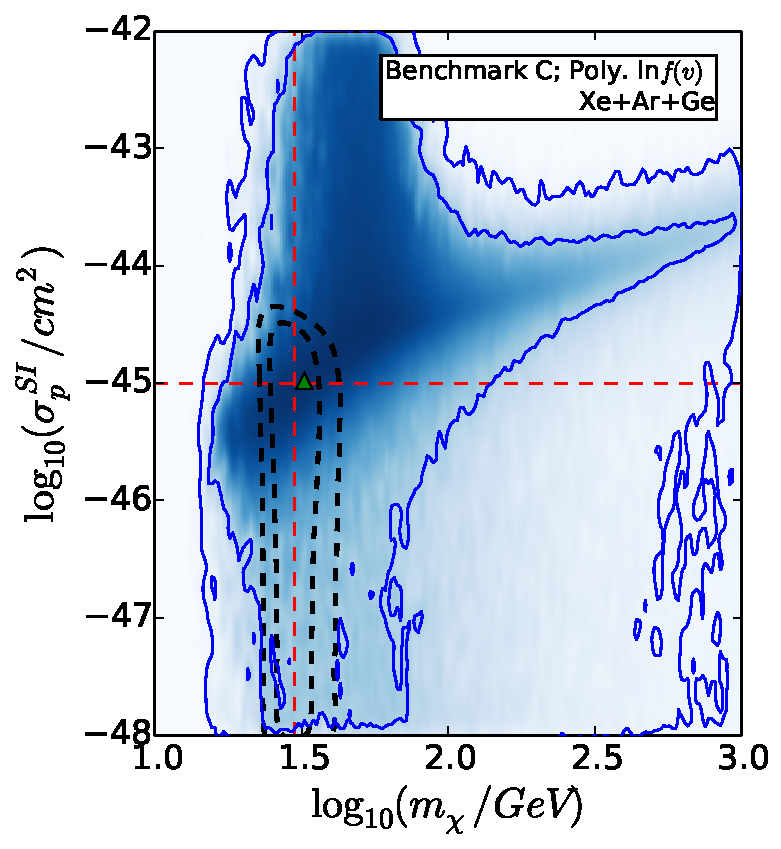
\includegraphics[width=0.32\textwidth]{NT/BenchmarkC_poly_noIC-mx_sigsi.pdf}
  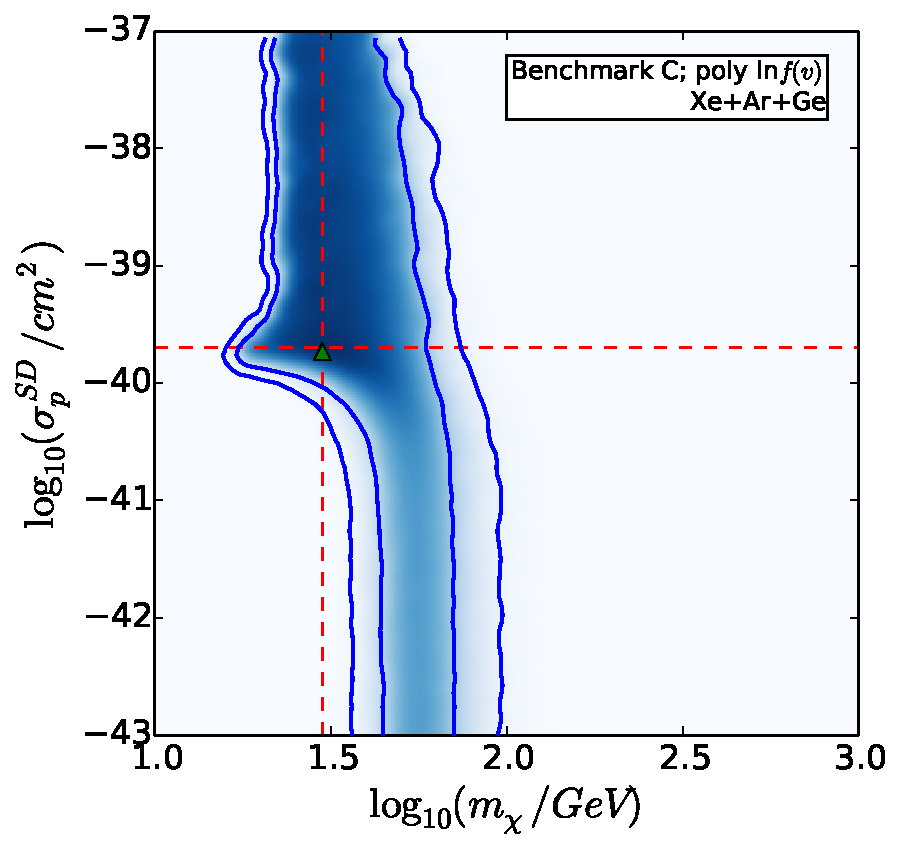
\includegraphics[width=0.32\textwidth]{NT/BenchmarkC_poly_noIC-mx_sigsd.pdf}
  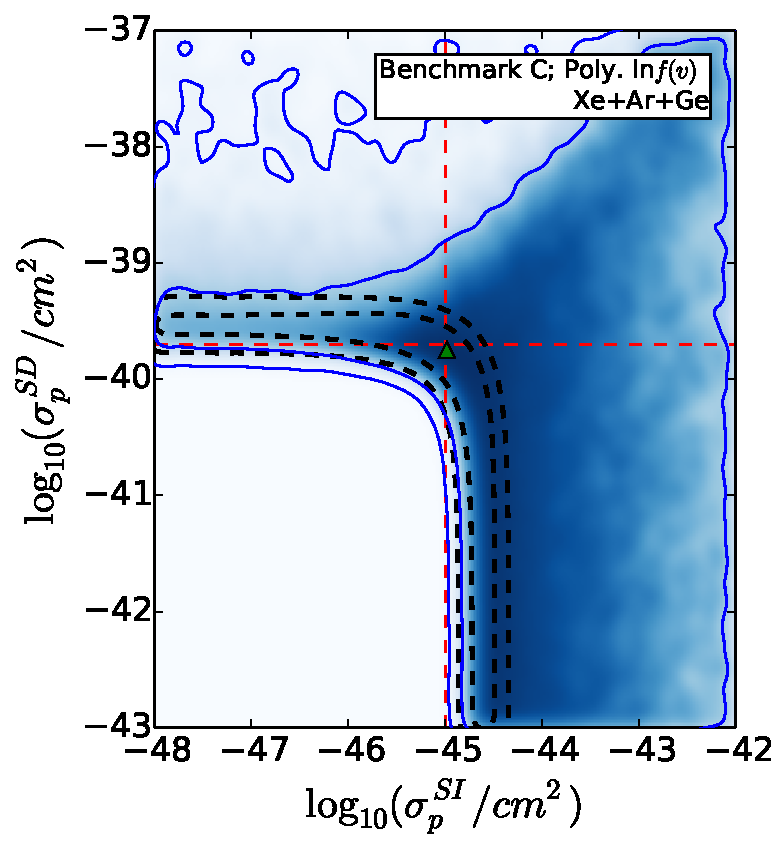
\includegraphics[width=0.32\textwidth]{NT/BenchmarkC_poly_noIC-sigsi_sigsd.pdf}

  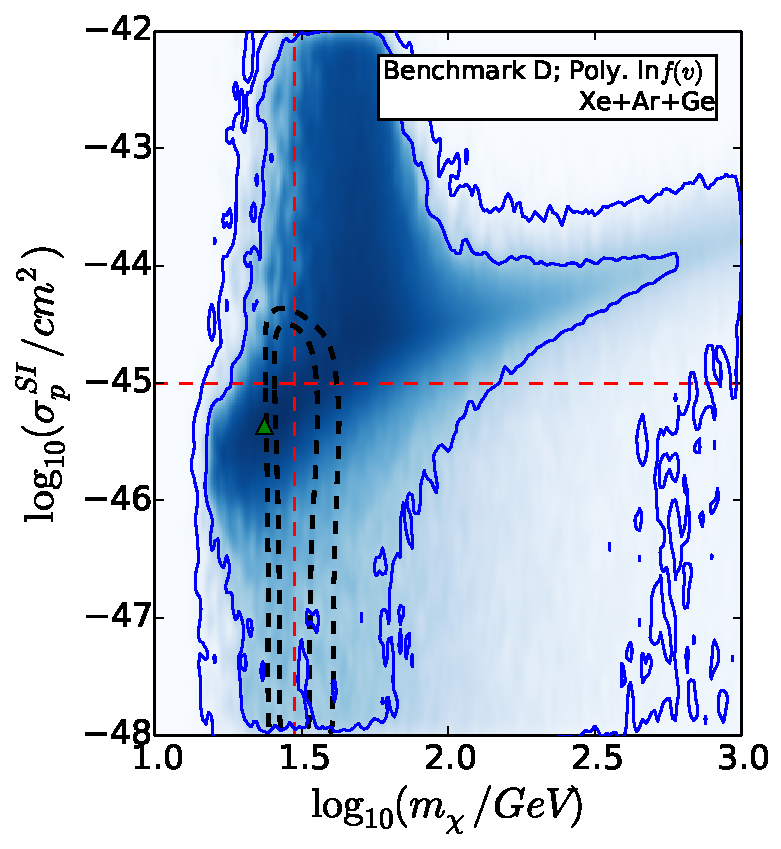
\includegraphics[width=0.32\textwidth]{NT/BenchmarkD_poly_noIC-mx_sigsi.pdf}
  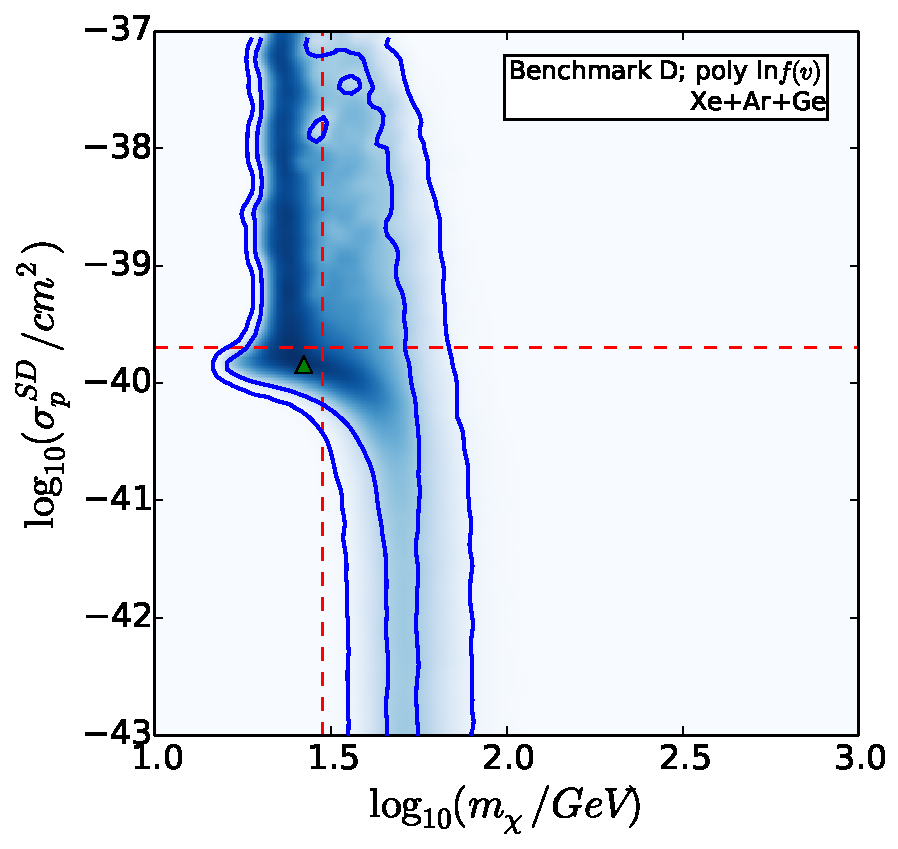
\includegraphics[width=0.32\textwidth]{NT/BenchmarkD_poly_noIC-mx_sigsd.pdf}
  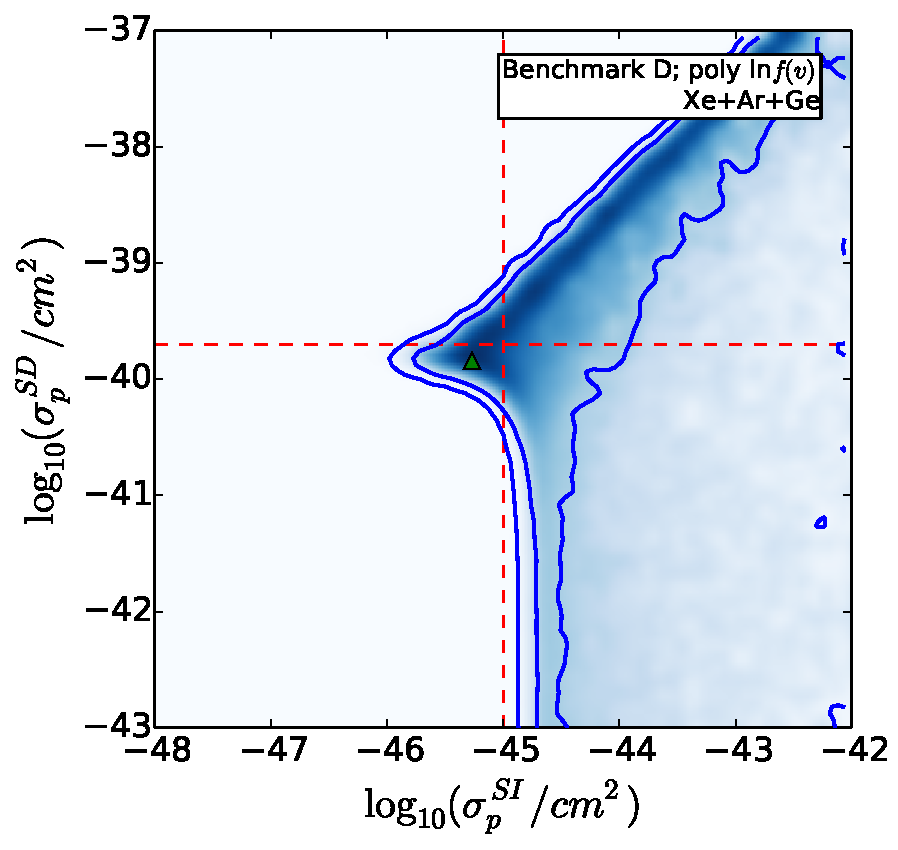
\includegraphics[width=0.32\textwidth]{NT/BenchmarkD_poly_noIC-sigsi_sigsd.pdf}
\caption{WHAT!}
\end{figure}


\section{Reconstructions with IceCube}
\label{sec:NT:withIC}

\begin{figure}[!ht]
  \centering
  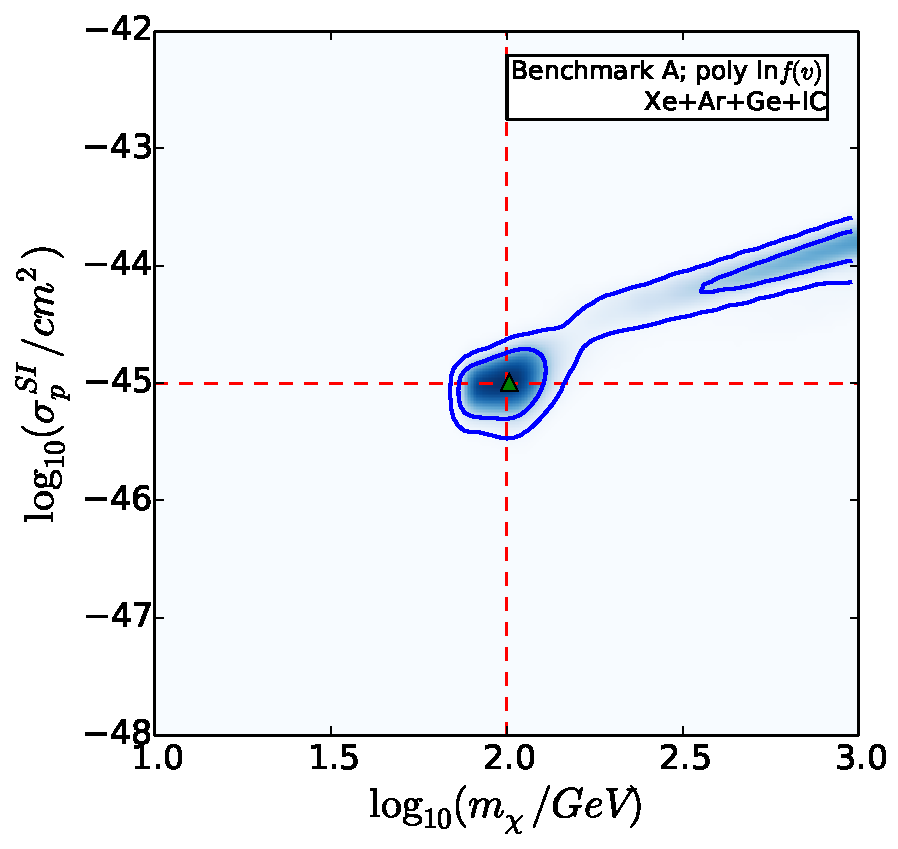
\includegraphics[width=0.32\textwidth]{NT/BenchmarkA_poly-mx_sigsi.pdf}
  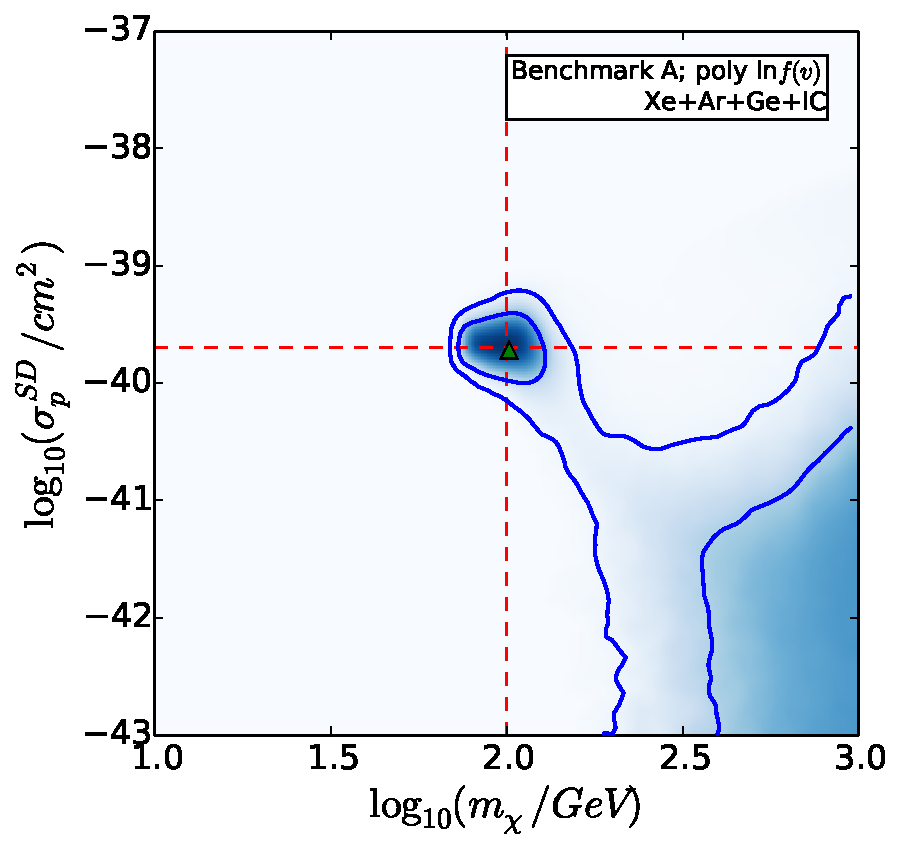
\includegraphics[width=0.32\textwidth]{NT/BenchmarkA_poly-mx_sigsd.pdf}
  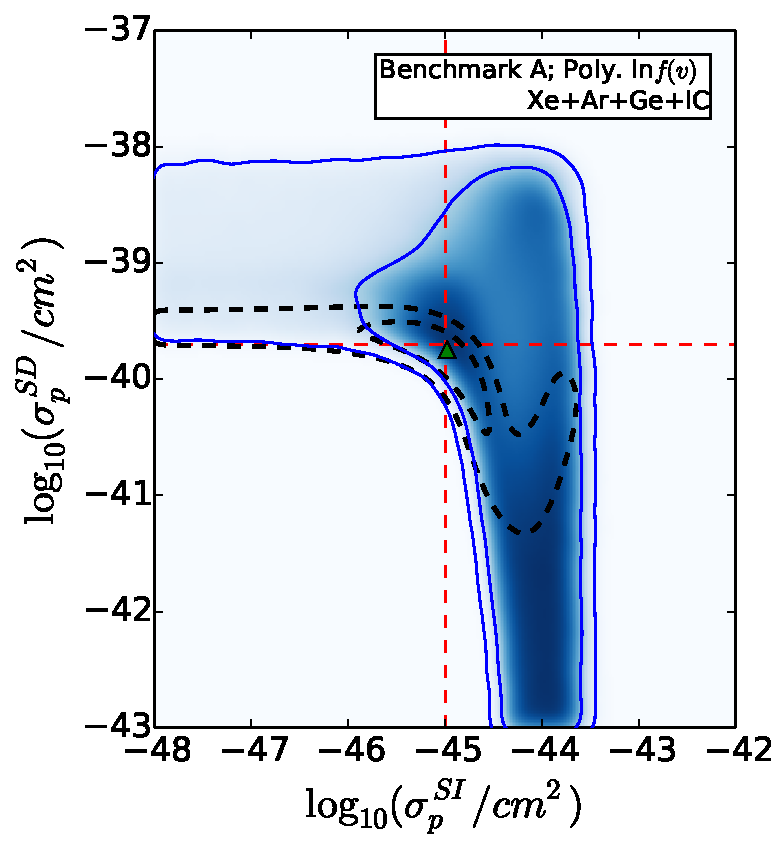
\includegraphics[width=0.32\textwidth]{NT/BenchmarkA_poly-sigsi_sigsd.pdf}

  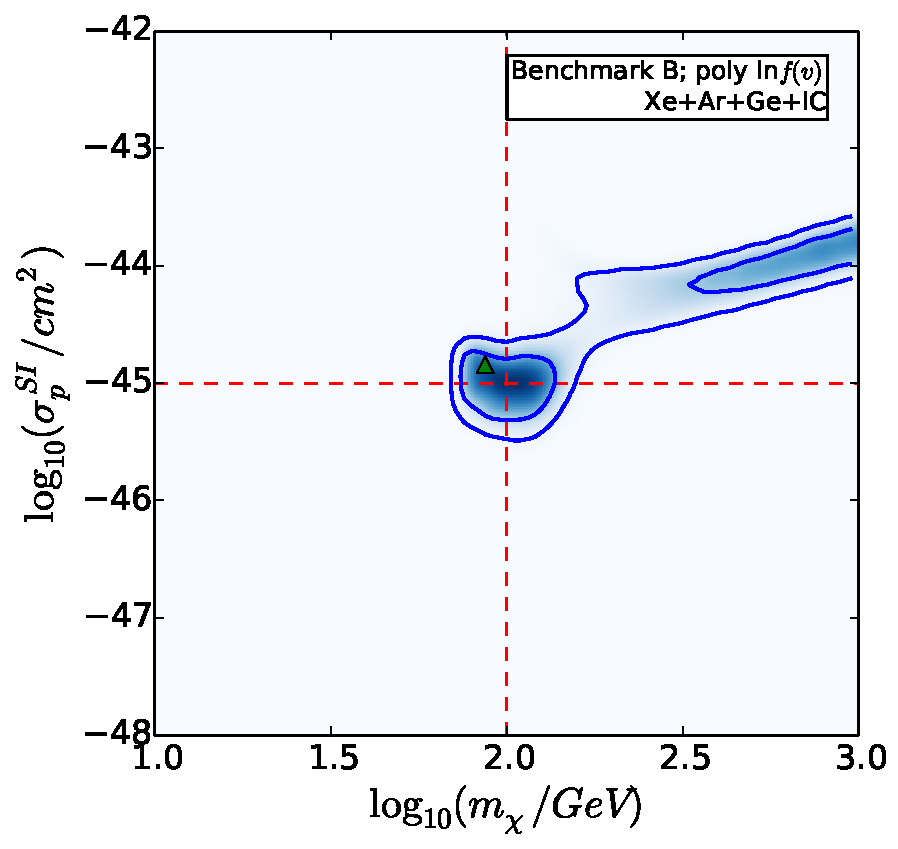
\includegraphics[width=0.32\textwidth]{NT/BenchmarkB_poly-mx_sigsi.pdf}
  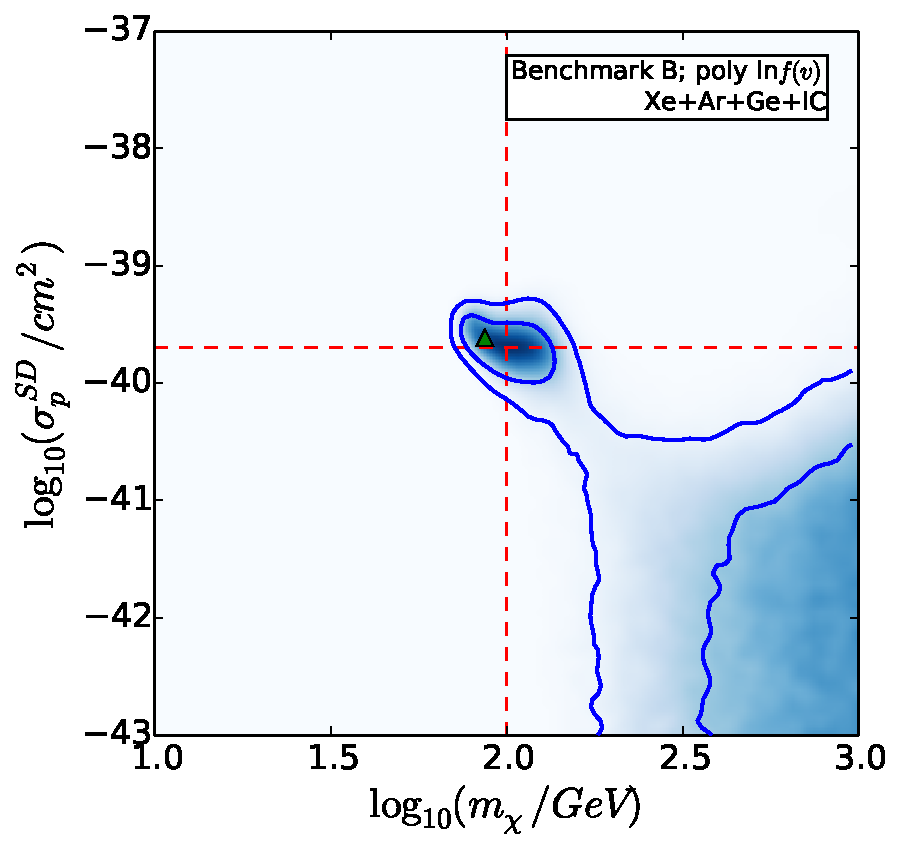
\includegraphics[width=0.32\textwidth]{NT/BenchmarkB_poly-mx_sigsd.pdf}
  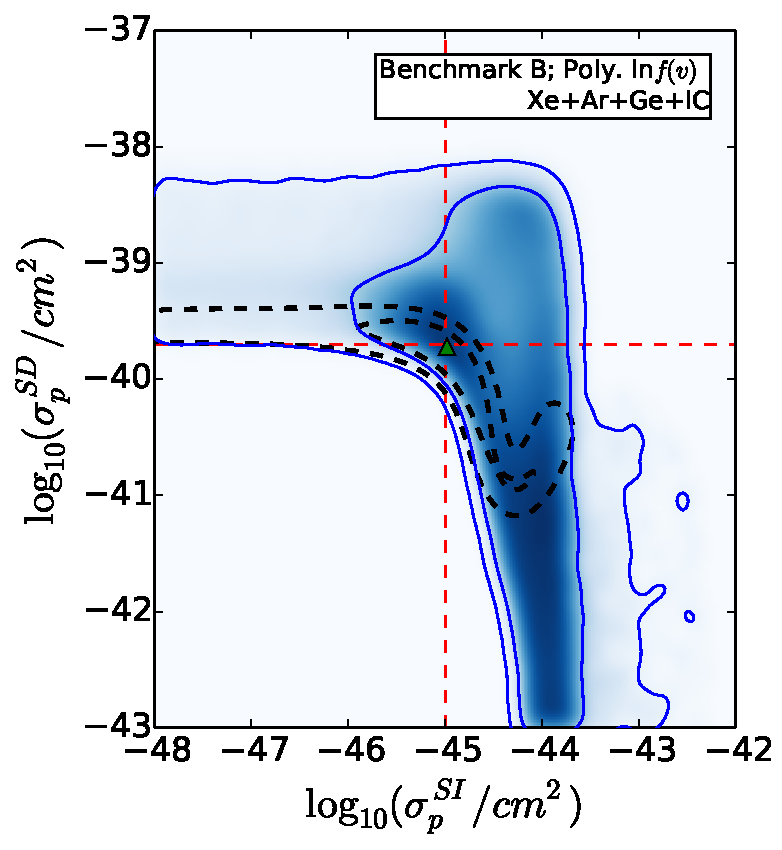
\includegraphics[width=0.32\textwidth]{NT/BenchmarkB_poly-sigsi_sigsd.pdf}

  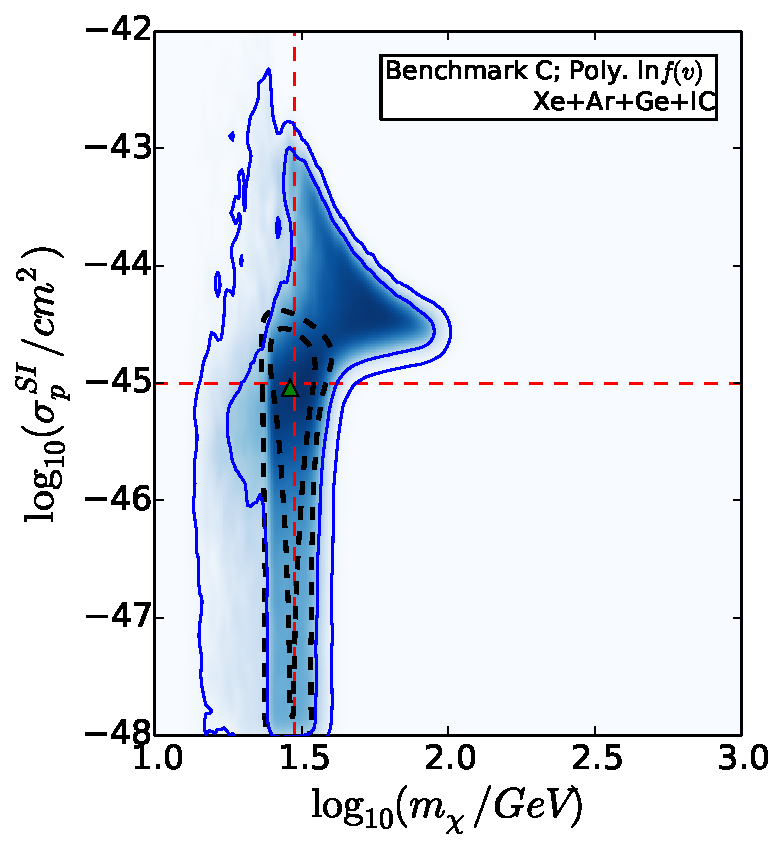
\includegraphics[width=0.32\textwidth]{NT/BenchmarkC_poly-mx_sigsi.pdf}
  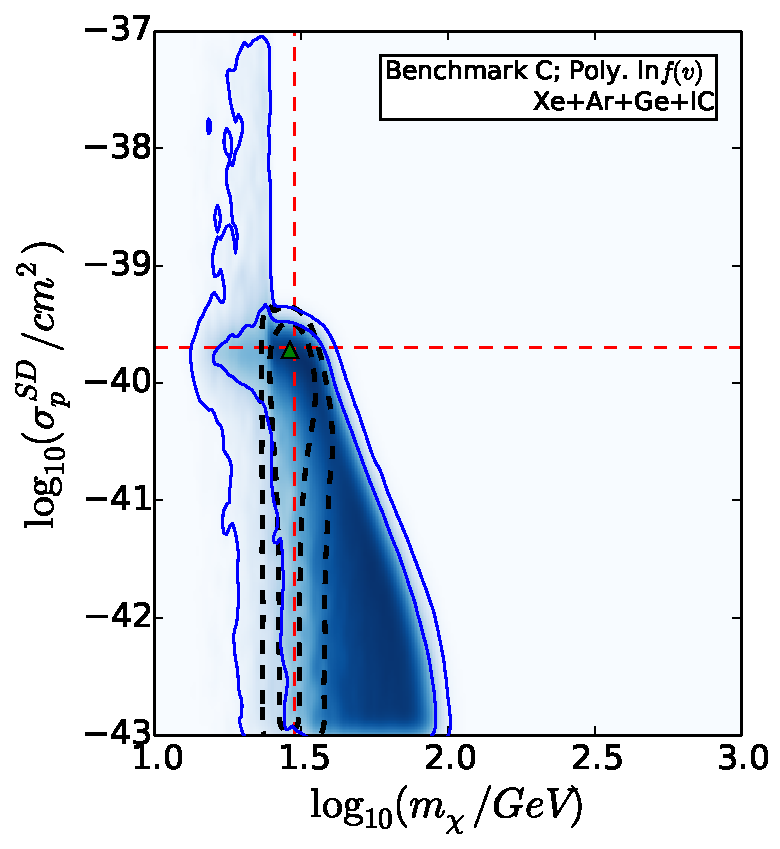
\includegraphics[width=0.32\textwidth]{NT/BenchmarkC_poly-mx_sigsd.pdf}
  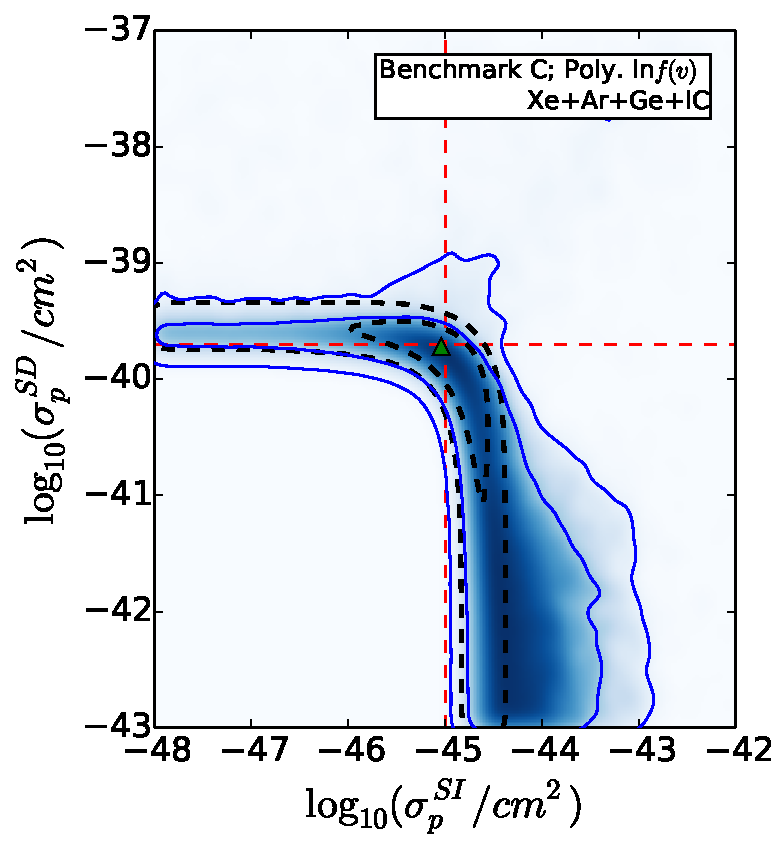
\includegraphics[width=0.32\textwidth]{NT/BenchmarkC_poly-sigsi_sigsd.pdf}

  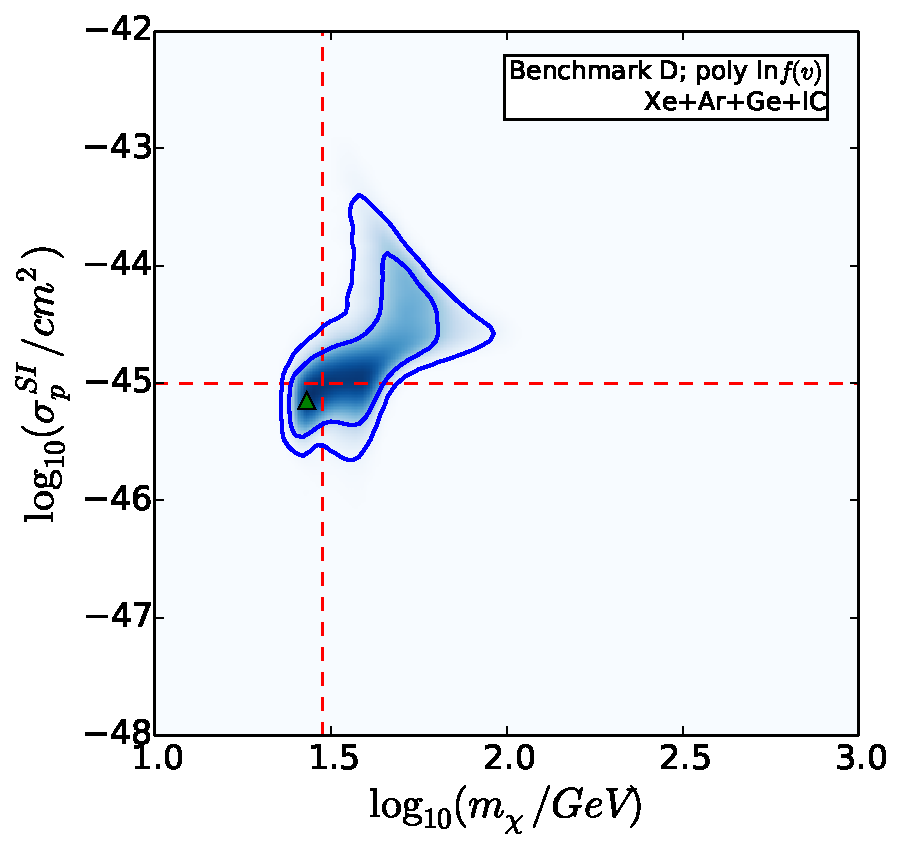
\includegraphics[width=0.32\textwidth]{NT/BenchmarkD_poly-mx_sigsi.pdf}
  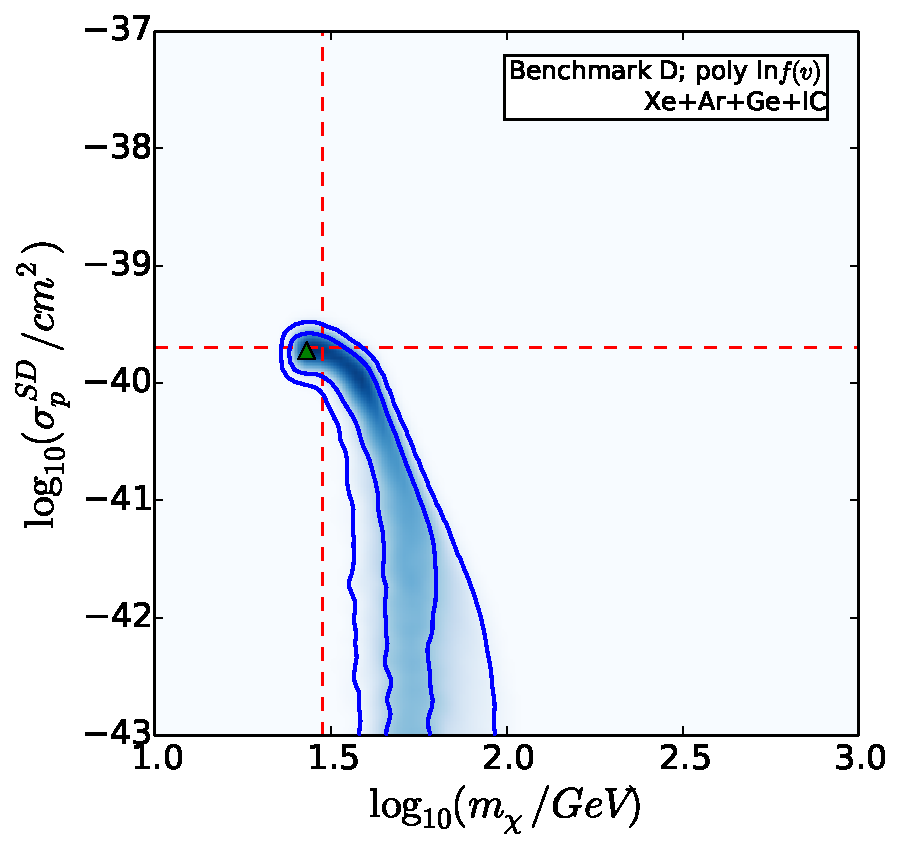
\includegraphics[width=0.32\textwidth]{NT/BenchmarkD_poly-mx_sigsd.pdf}
  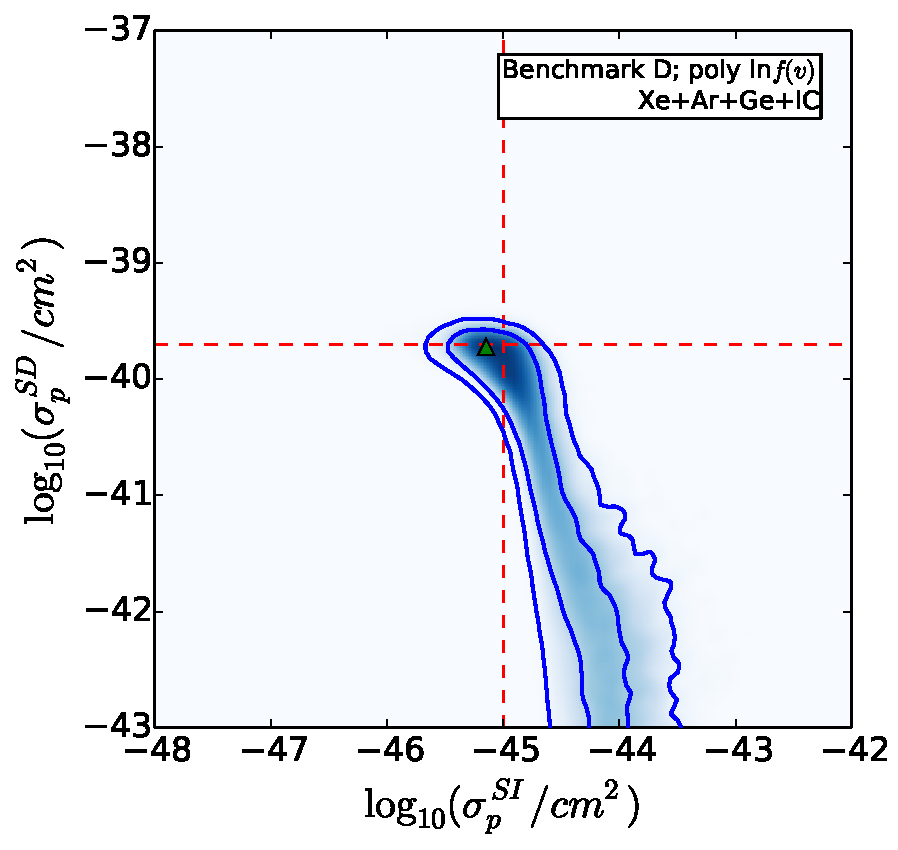
\includegraphics[width=0.32\textwidth]{NT/BenchmarkD_poly-sigsi_sigsd.pdf}
\caption{WHAT!}
\end{figure}

